\documentclass{llncs}
\usepackage{fullpage}

%load needed packages
\usepackage{graphicx}
\usepackage{array}
\usepackage{booktabs}
\usepackage[utf8]{inputenc}
\usepackage{amsmath} 


\begin{document}

\title{Task A}
\subtitle{Supervised Learning Model Evaluation Metrics}

\author{Diego De Pablo}
\institute{\email{depablodiego@uma.es} \\
Health Engineering. Málaga University.}

\maketitle 

\vspace{1cm} % Space down the title

\textit{
	This work investigates the performance of various classification methods in a supervised learning context, focusing on how certain techniques can yield misleadingly high metrics. Specifically, some methods that classify all samples into a single category may achieve better performance metrics compared to methods that accurately differentiate between positive and negative samples. The analysis highlights the importance of robust metrics like the Jaccard index and F-measure, which provide valuable insights into model performance. Ultimately, it underscores the necessity of understanding the specific goals of the analysis to determine which metrics are most relevant for evaluating a model’s effectiveness. }



\section{Introduction}

Artificial intelligence (AI) has emerged as a transformative solution to numerous challenges in a wide range of domains, often being viewed as a key to simple and efficient problem-solving. However, the performance of AI models must be critically assessed to understand their real-world applicability and limitations. In particular, supervised learning algorithms are often used in classification tasks, where the performance of these models can be evaluated through specific metrics.

In this work, we explore the key performance metrics derived from the \textit{confusion matrix} to assess and compare supervised learning models. These metrics include \textbf{Precision}, \textbf{Recall}, \textbf{Specificity}, \textbf{False Positive Rate}, \textbf{False Negative Rate}, \textbf{Accuracy}, \textbf{Spatial Accuracy}, \textbf{Jaccard Index}, and \textbf{F-measure}. These metrics are commonly used to provide a detailed view of a model’s performance across different dimensions. By understanding and comparing these metrics, we can gain insights into the strengths and weaknesses of the classification methods being evaluated.

In computational learning, applying classification algorithms to predict disease progression is critical for deriving meaningful insights from complex biomedical data. The primary focus of this project is to evaluate and compare the performance of several classification methods using a dataset relevant to disease classification. The analysis will focus on various aspects, including the dataset's class distribution, balance, and overall characteristics, and will use a range of well-established performance metrics.

The metrics used in this analysis provide a quantitative basis to assess each model’s strengths and limitations, allowing us to determine which algorithm performs best for predicting outcomes in the dataset. Specifically, we will implement an algorithm to calculate several well-known metrics based on the number of \textbf{True Positives (TP)}, \textbf{True Negatives (TN)}, \textbf{False Positives (FP)}, and \textbf{False Negatives (FN)}. 

These metrics will enable a comprehensive evaluation of each method's effectiveness in predicting for example disease progression. Furthermore, graphical representations, such as heatmaps and radar charts, will be used to provide a visual comparison of the methods. This will facilitate better understanding of each model's advantages and limitations, allowing for more informed decision-making when selecting the appropriate classification model.

\section{Dataset Description}

The aim of this work is to highlight the validation methods and explore examples ranging from realistic to exaggerated cases that, in certain scenarios, might be considered good results if certain metrics are ignored. Even though these results may seem favorable, they can actually be misleading. To demonstrate this, we will base our analysis on the following dataset (observe the figure \ref{fig:dataset}).

\begin{figure}[h!]
	\begin{center}  % Usamos el entorno 'center'
		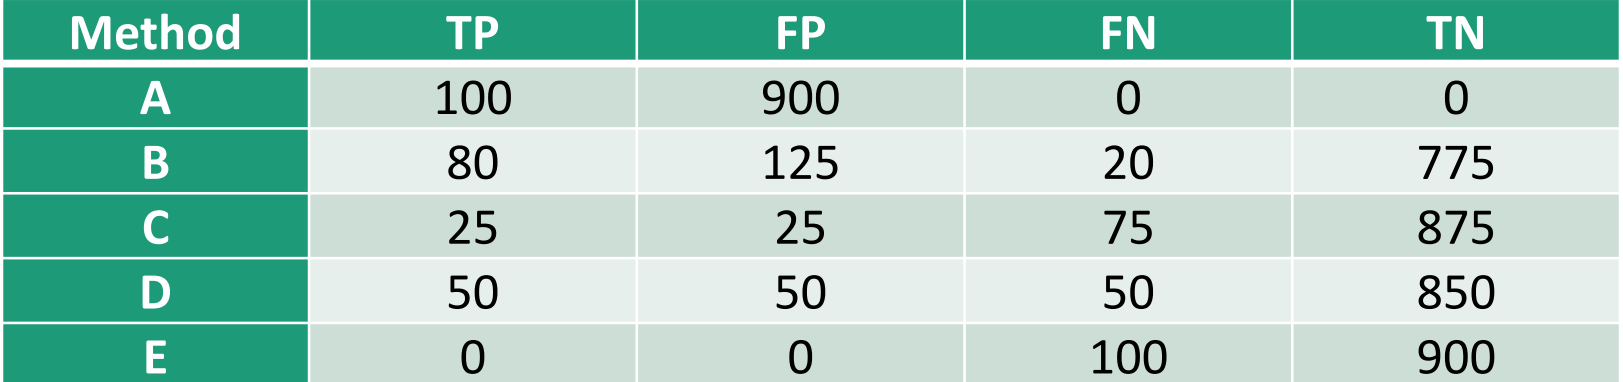
\includegraphics[width=1\textwidth]{images/dataset.png}
		\caption{The methods studied in this work}
		\label{fig:dataset}
	\end{center}
\end{figure}

\vspace{-20pt} % Ajusta este valor para reducir el espacio

The five hypothetical methods in this study are evaluated on a dataset of \textbf{1000 samples}, divided into \textbf{two classes} (positive or negative). This dataset is notably \textbf{imbalanced}, with 100 positive and 900 negative samples, which can lead to biased models and misleading metrics, as seen with methods A and E that perform poorly on specific measures.

Imbalanced datasets skew results, making some models appear more effective than they are. Techniques such as \textbf{oversampling}, \textbf{undersampling}, and \textbf{weight adjustment} are used to mitigate these effects, ensuring more reliable evaluations.

Figure \ref{fig:confusion} illustrates the percentage confusion matrix for each method, alongside a sixth matrix representing a perfect model that correctly identifies all positive and negative samples.



\begin{figure}[h!]
	\begin{center}  % Usamos el entorno 'center'
		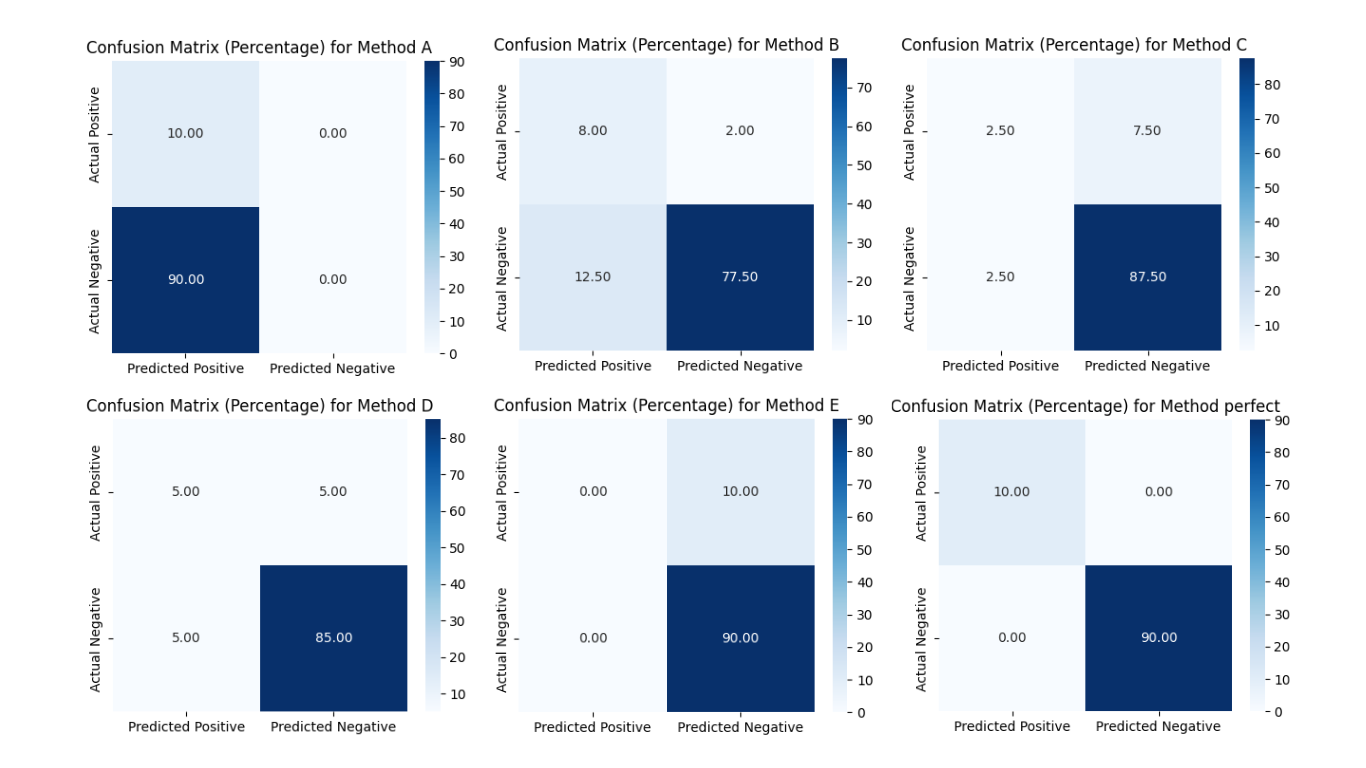
\includegraphics[width=1\textwidth]{images/5_metodos.png}
		\caption{6 confusion matrices, from A to E and the case of the perfect confusion matrix for this dataset}
		\label{fig:confusion}
	\end{center}
\end{figure}

Examining the confusion matrix for each method in relation to the ideal confusion matrix for the dataset reveals significant shortcomings in methods A and E, which classify all samples as either positive or negative. In contrast, methods B, C, and D demonstrate more realistic classification patterns, aligning more closely with the expectations of an effective machine learning approach. Although these methods approach the performance of a perfect model, they still exhibit a small percentage of false positives and false negatives. To determine which of these three methods is superior, it is essential to consider additional factors, such as validation metrics and the specific objectives for which the model is intended.

\section{Metrics Overview}

In this work, we implemented a function to compute various validation metrics using the true positives (TP), false positives (FP), true negatives (TN), and false negatives (FN) yielded by each method. The results are visualized in a heatmap  (see the Figure \ref{fig:heatmap}) to clearly present the performance of each method.

\begin{figure}[h!]
	\begin{center}  % Usamos el entorno 'center'
		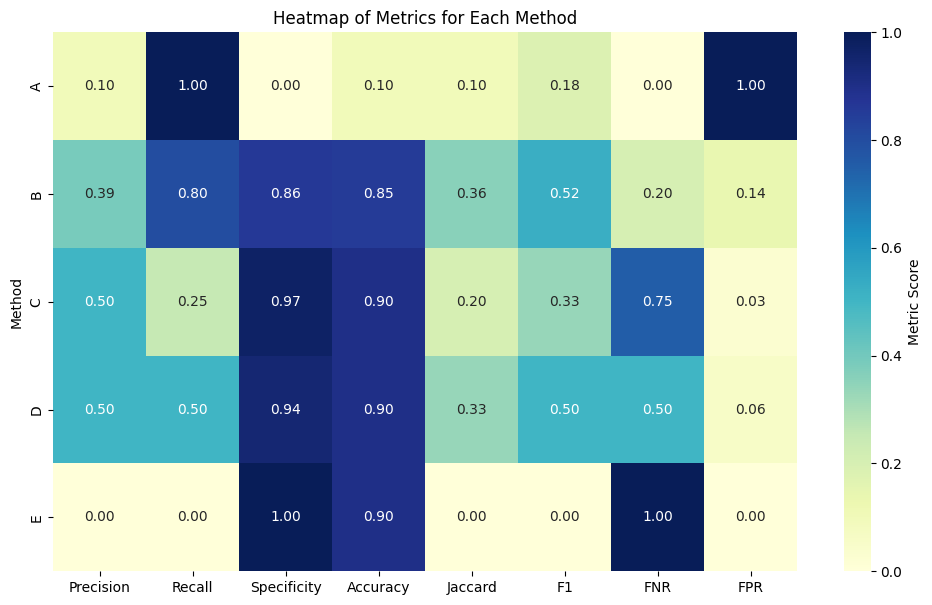
\includegraphics[width=1\textwidth]{images/heat_map.png}
		\caption{The methods studied in this work}
		\label{fig:heatmap}
	\end{center}
\end{figure}

\subsection{Summary of Expected Ranges}
\begin{itemize}
	\item Precision, Recall, Specificity, Accuracy, Jaccard, F1: Values range from 0 to 1, with higher values indicating better performance.
	\item FNR, FPR: Values range from 0 to 1, with lower values indicating better performance.
\end{itemize}


\subsection{Evaluation Metrics}

In machine learning, evaluation metrics are crucial for assessing model performance, particularly in classification tasks. Each metric provides unique insights into various aspects of the model's predictions. Below is a breakdown of the key metrics used in this study:

\subsubsection{Precision (PR)}
\textit{PR = TP / (TP + FP)} - Indicates how many of the predicted positives were actually correct. It is especially useful when false positives are costly, such as in spam detection.

\begin{table}[h]
	\centering
	\begin{tabular}{|c|c|c|c|c|c|}
		\hline
		\textbf{Metric} & \textbf{A} & \textbf{B} & \textbf{C} & \textbf{D} & \textbf{E} \\ 
		\hline
		\textbf{Precision} & 0.1000 & 0.3902 & 0.5000 & 0.5000 & 0.0000 \\ 
		\hline
	\end{tabular}
	\caption{Precision metrics for each method.}
	\label{tab:precision}
\end{table}

\vspace{-20pt} % Ajusta este valor para reducir el espacio

\subsubsection{Recall (RC)}
\textit{RC = TP / (TP + FN)} - Measures how many actual positives were correctly identified. High recall is critical in scenarios where missing a positive case is costly, like medical diagnoses.

\subsubsection{Specificity (SP)}
\textit{SP = TN / (TN + FP)} - Represents the proportion of actual negatives that were correctly identified. It is valuable in fraud detection, minimizing false positives.

\subsubsection{Accuracy (ACC)}
\textit{ACC = (TN + TP) / (TP + FN + FP + TN)} - Measures the overall proportion of correct predictions but can be misleading with imbalanced datasets.

\subsubsection{Spatial Accuracy (S) or Jaccard Index (J)}
\textit{J = TP / (TP + FN + FP)} - Evaluates the overlap between predicted and actual positives, often used in image segmentation tasks.

\subsubsection{F-measure (Fm)}
\textit{Fm = (2 * PR * RC) / (PR + RC)} - The harmonic mean of precision and recall, balancing their trade-offs, especially useful in binary classification with imbalanced datasets.

\subsubsection{False Negative Rate (FNR)}
\textit{FNR = FN / (TP + FN)} - Reflects the proportion of actual positives incorrectly predicted as negatives. Crucial when false negatives carry significant consequences.

\subsubsection{False Positive Rate (FPR)}
\textit{FPR = FP / (FP + TN)} - Indicates the proportion of actual negatives incorrectly classified as positives. Important in tasks like fraud detection, where maintaining a low FPR is essential.



\section{Metrics Overview}

In the methods that we will evaluate we have the results of the confusion matrix, that is, \textbf{True Positives (TP)}, \textbf{True Negatives (TN)}, \textbf{False Positives (FP)}, and \textbf{False Negatives (FN)}, and with this data we can obtain the following metrics:

\subsection{Precision}
Precision, also known as positive predictive value, measures the proportion of true positive predictions out of all positive predictions made by the model. It provides insight into the model’s ability to avoid false positives.
\[
Precision = \frac{TP}{TP + FP}
\]

\subsection{Recall}
Recall, or sensitivity, measures the proportion of actual positives that are correctly identified by the model. It is particularly useful in scenarios where minimizing false negatives is critical.
\[
Recall = \frac{TP}{TP + FN}
\]

\subsection{Specificity}
Specificity quantifies the model's ability to correctly identify negatives (i.e., true negatives) out of all actual negatives.
\[
Specificity = \frac{TN}{TN + FP}
\]

\subsection{False Positive Rate}
This metric measures the proportion of false positives out of all actual negatives, indicating how often the model incorrectly classifies a negative instance as positive.
\[
FPR = \frac{FP}{FP + TN}
\]

\subsection{False Negative Rate}
The false negative rate measures the proportion of false negatives out of all actual positives, highlighting the rate at which the model misses positive cases.
\[
FNR = \frac{FN}{TP + FN}
\]

\subsection{Accuracy}
Accuracy measures the proportion of correct predictions (both true positives and true negatives) out of the total predictions made.
\[
Accuracy = \frac{TP + TN}{TP + FP + FN + TN}
\]

\subsection{Jaccard Index}
Also referred to as spatial accuracy, the Jaccard Index quantifies the similarity between the predicted and actual positive classes.
\[
Jaccard = \frac{TP}{TP + FN + FP}
\]

\subsection{F-measure}
The F-measure is the harmonic mean of precision and recall, providing a balanced metric that considers both false positives and false negatives.
\[
F1 = \frac{2 \cdot Precision \cdot Recall}{Precision + Recall}
\]


 
\section{Conclusions}
 
In this study, we conducted a comprehensive comparison of three clustering algorithms applied to a yeast sporulation dataset. The K-means algorithm, with K=2, demonstrated superior performance in terms of cluster compactness and separation, outperforming both hierarchical clustering and self-organizing maps. Nevertheless, each clustering method brings its own strengths and may perform better under different conditions or datasets. It is also crucial to consider the advancements in clustering methodologies and technology over time. By comparing our results to an older study, we observed that modern algorithms and computational power significantly enhance the quality of clustering outcomes, emphasizing the importance of continuous innovation in data analysis techniques.

\bibliographystyle{plain}  % Puedes cambiar "plain" por el estilo de tu preferencia, como apalike, ieeetr, etc.
\bibliography{bibliography}  % Aquí va el nombre de tu archivo .bib (sin la extensión .bib)
\end{document}
